% Licensed under the Creative Commons Attribution Share Alike 4.0 International.
% See the LICENSE file in the repository root for full license text.

\section{认识计算机}

现在是 2022 年,微型计算机(简称为计算机)无处不在,捞钱的概念的层出不穷。但不管那些人用何种方式捞钱,只要涉及计算机,就一定离不开冯·诺依曼计算机。

计算机的核心必然是数字电路,但现在的程序员需要知道计算机中的任何逻辑门\footnote{逻辑门是组成数字电路的基本元件。}吗?显然不需要,否则会写程序的小学生的数量将大幅减少。\textbf{冯·诺依曼体系结构的杰出贡献之一,便是将计算机的逻辑结构抽象出来,但其设计又可以被数字电路实现。}冯·诺依曼计算机的体系结构如图 \ref{pic:logic-computer}\footnote{图源:北京大学《微处理器与接口技术》课件。} 所示。

\begin{figure}[H]
	\centering
	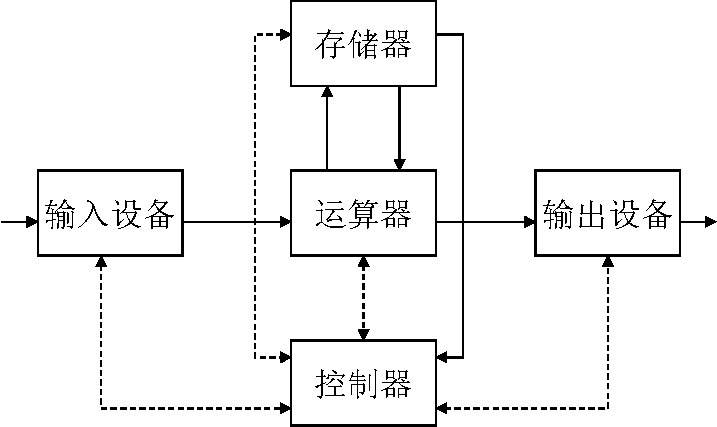
\includegraphics[width=0.45\linewidth]{pic/logic-computer.pdf}
	\caption{冯·诺依曼体系结构}
	\label{pic:logic-computer}
\end{figure}

冯·诺依曼计算机由控制器、运算器、存储器、输入设备、输出设备组成,是一台抽象的计算机。除了抽象性这一贡献,冯·诺依曼计算机还具有存储程序的优点,这使得计算机的运行速度大幅提高:想象一下写有程序的纸带被老式计算机一点点拉扯,速度能快吗?图 \ref{pic:paper-tape}\footnote{图源:liangshuang,《操作系统的发展史》,博客园,\url{https://www.cnblogs.com/ls13691357174/p/10485469.html}。} 展示了一条写有程序的纸带;今天,我们写程序一般都敲键盘。一旦程序编写完成,它将飞速运行,运行速度与你的手速无关。

\begin{figure}[ht]
	\centering
	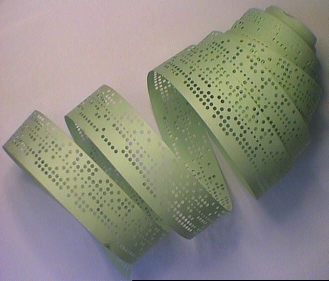
\includegraphics[width=0.5\linewidth]{pic/paper-tape.png}
	\caption{写有程序的纸带}
	\label{pic:paper-tape}
\end{figure}

\textbf{存储程序、程序控制执行}是冯·诺依曼计算机的工作方式。“存储程序”指将程序像数据一样存储到计算机内部存储器中,而“程序控制执行”指明了计算机使用程序的方法:将编制好的程序放入存储器后,首先执行第一条指令,之后周而复始地取出指令、分析指令、执行指令。

图 \ref{pic:asm} 展示了存储程序和程序控制执行在真实计算机中的表现。图中,Bytes 列是汇编程序 Opcode 在内存中存储的数据(称为机器码),而 Address 列中的 \lstinline{>>} 符号则表示当前正在执行的指令\footnote{当程序是这种可以和机器码直接对应的汇编程序时,称单行程序为一条指令。CPU 一般一次只处理一条指令。}。

\begin{figure}[ht]
	\centering
	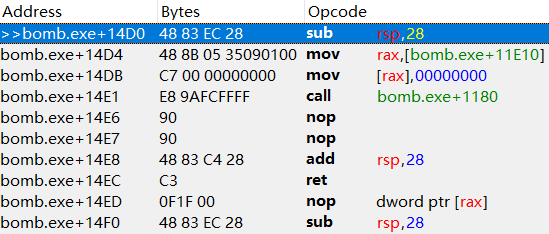
\includegraphics[width=0.75\linewidth]{pic/asm-1.png}
	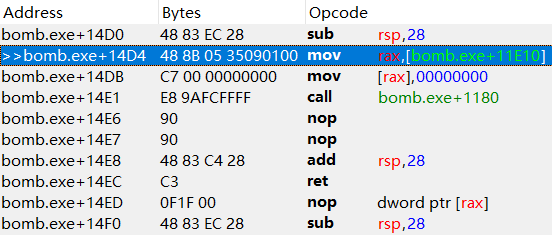
\includegraphics[width=0.75\linewidth]{pic/asm-2.png}
	\caption{存储程序与程序控制执行}
	\label{pic:asm}
\end{figure}

常见的真实计算机最重要的部分为大家熟知的中央处理器(Central Processing Unit, CPU),图 \ref{pic:asm} 中的指令均由 CPU 执行。但单一的 CPU 无法构成符合冯·诺依曼体系结构的系统,必须辅以外部\footnote{此处的外部相对于 CPU 而言。我们常称其中一种外部存储器为内存。}的存储器以及输入输出接口才能构成完整的计算机。图 \ref{pic:computer}\footnote{图源:北京大学《微处理器与接口技术》课件。} 展示了计算机的结构。

\begin{figure}[ht]
	\centering
	\begin{minipage}{0.45\linewidth}
		\centering
		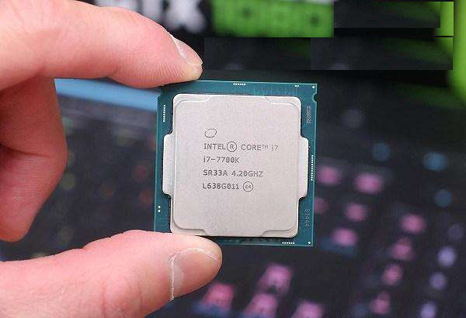
\includegraphics[width=0.95\linewidth]{pic/cpu-1.png}
	\end{minipage}
	\begin{minipage}{0.45\linewidth}
		\centering
		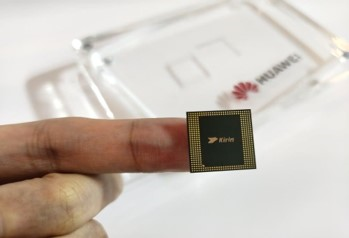
\includegraphics[width=0.95\linewidth]{pic/cpu-2.png}
	\end{minipage}
	\caption{常见的 CPU}
	\label{pic:cpu}
\end{figure}

\begin{figure}[ht]
	\centering
	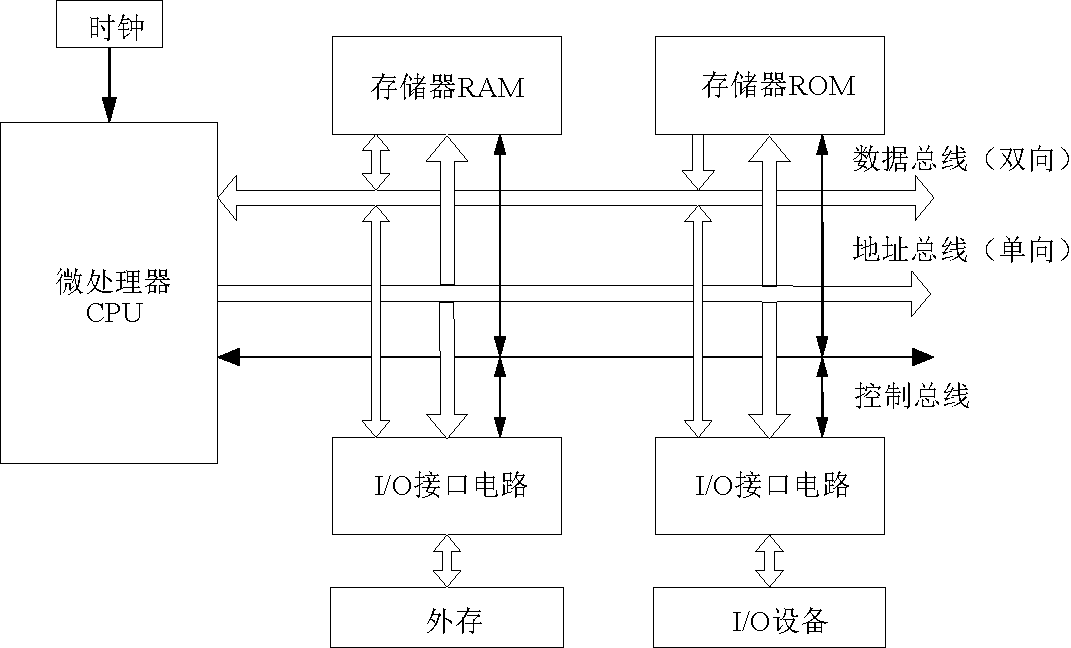
\includegraphics[width=0.8\linewidth]{pic/computer.pdf}
	\caption{计算机的结构}
	\label{pic:computer}
\end{figure}

现代的计算机不断向快速化和小型化发展。目前,CPU 真实架构中的缓存、流水、多核等概念,已经无法用纯粹的冯·诺依曼体系结构解释;为了减少外设数量,缩减电路板尺寸,出现了将 CPU 和存储器集成在一块芯片上的单片机,常用于控制领域。无论怎样发展,图 \ref{pic:computer} 所示的结构仍然成立,之后的内容也仍然适用,因为\textbf{这些发展对于通用的程序设计原则而言应当是透明的\footnote{计算机领域的透明指“看不见”,而不是“可以透过看见”。}(Transparent)}。如果需要充分利用新结构带来的速度优势,则势必涉及专有的内容,例如,可以使用 CPU 提供的扩展指令集加速数据的处理,但据此设计的程序必然只能在少量支持该指令集的处理器上运行;当然这也超出了我们的讨论范围。另外,我们常说使用图形处理器(Graphics Processing Unit, GPU)进行加速,它们实际上属于外部设备,仍然需要通过输入输出接口由 CPU 进行控制。

\clearpage